\begin{figure}[!t]
    \centering
    
    % Row 1
    \begin{subfigure}{0.48\textwidth}
        \centering
        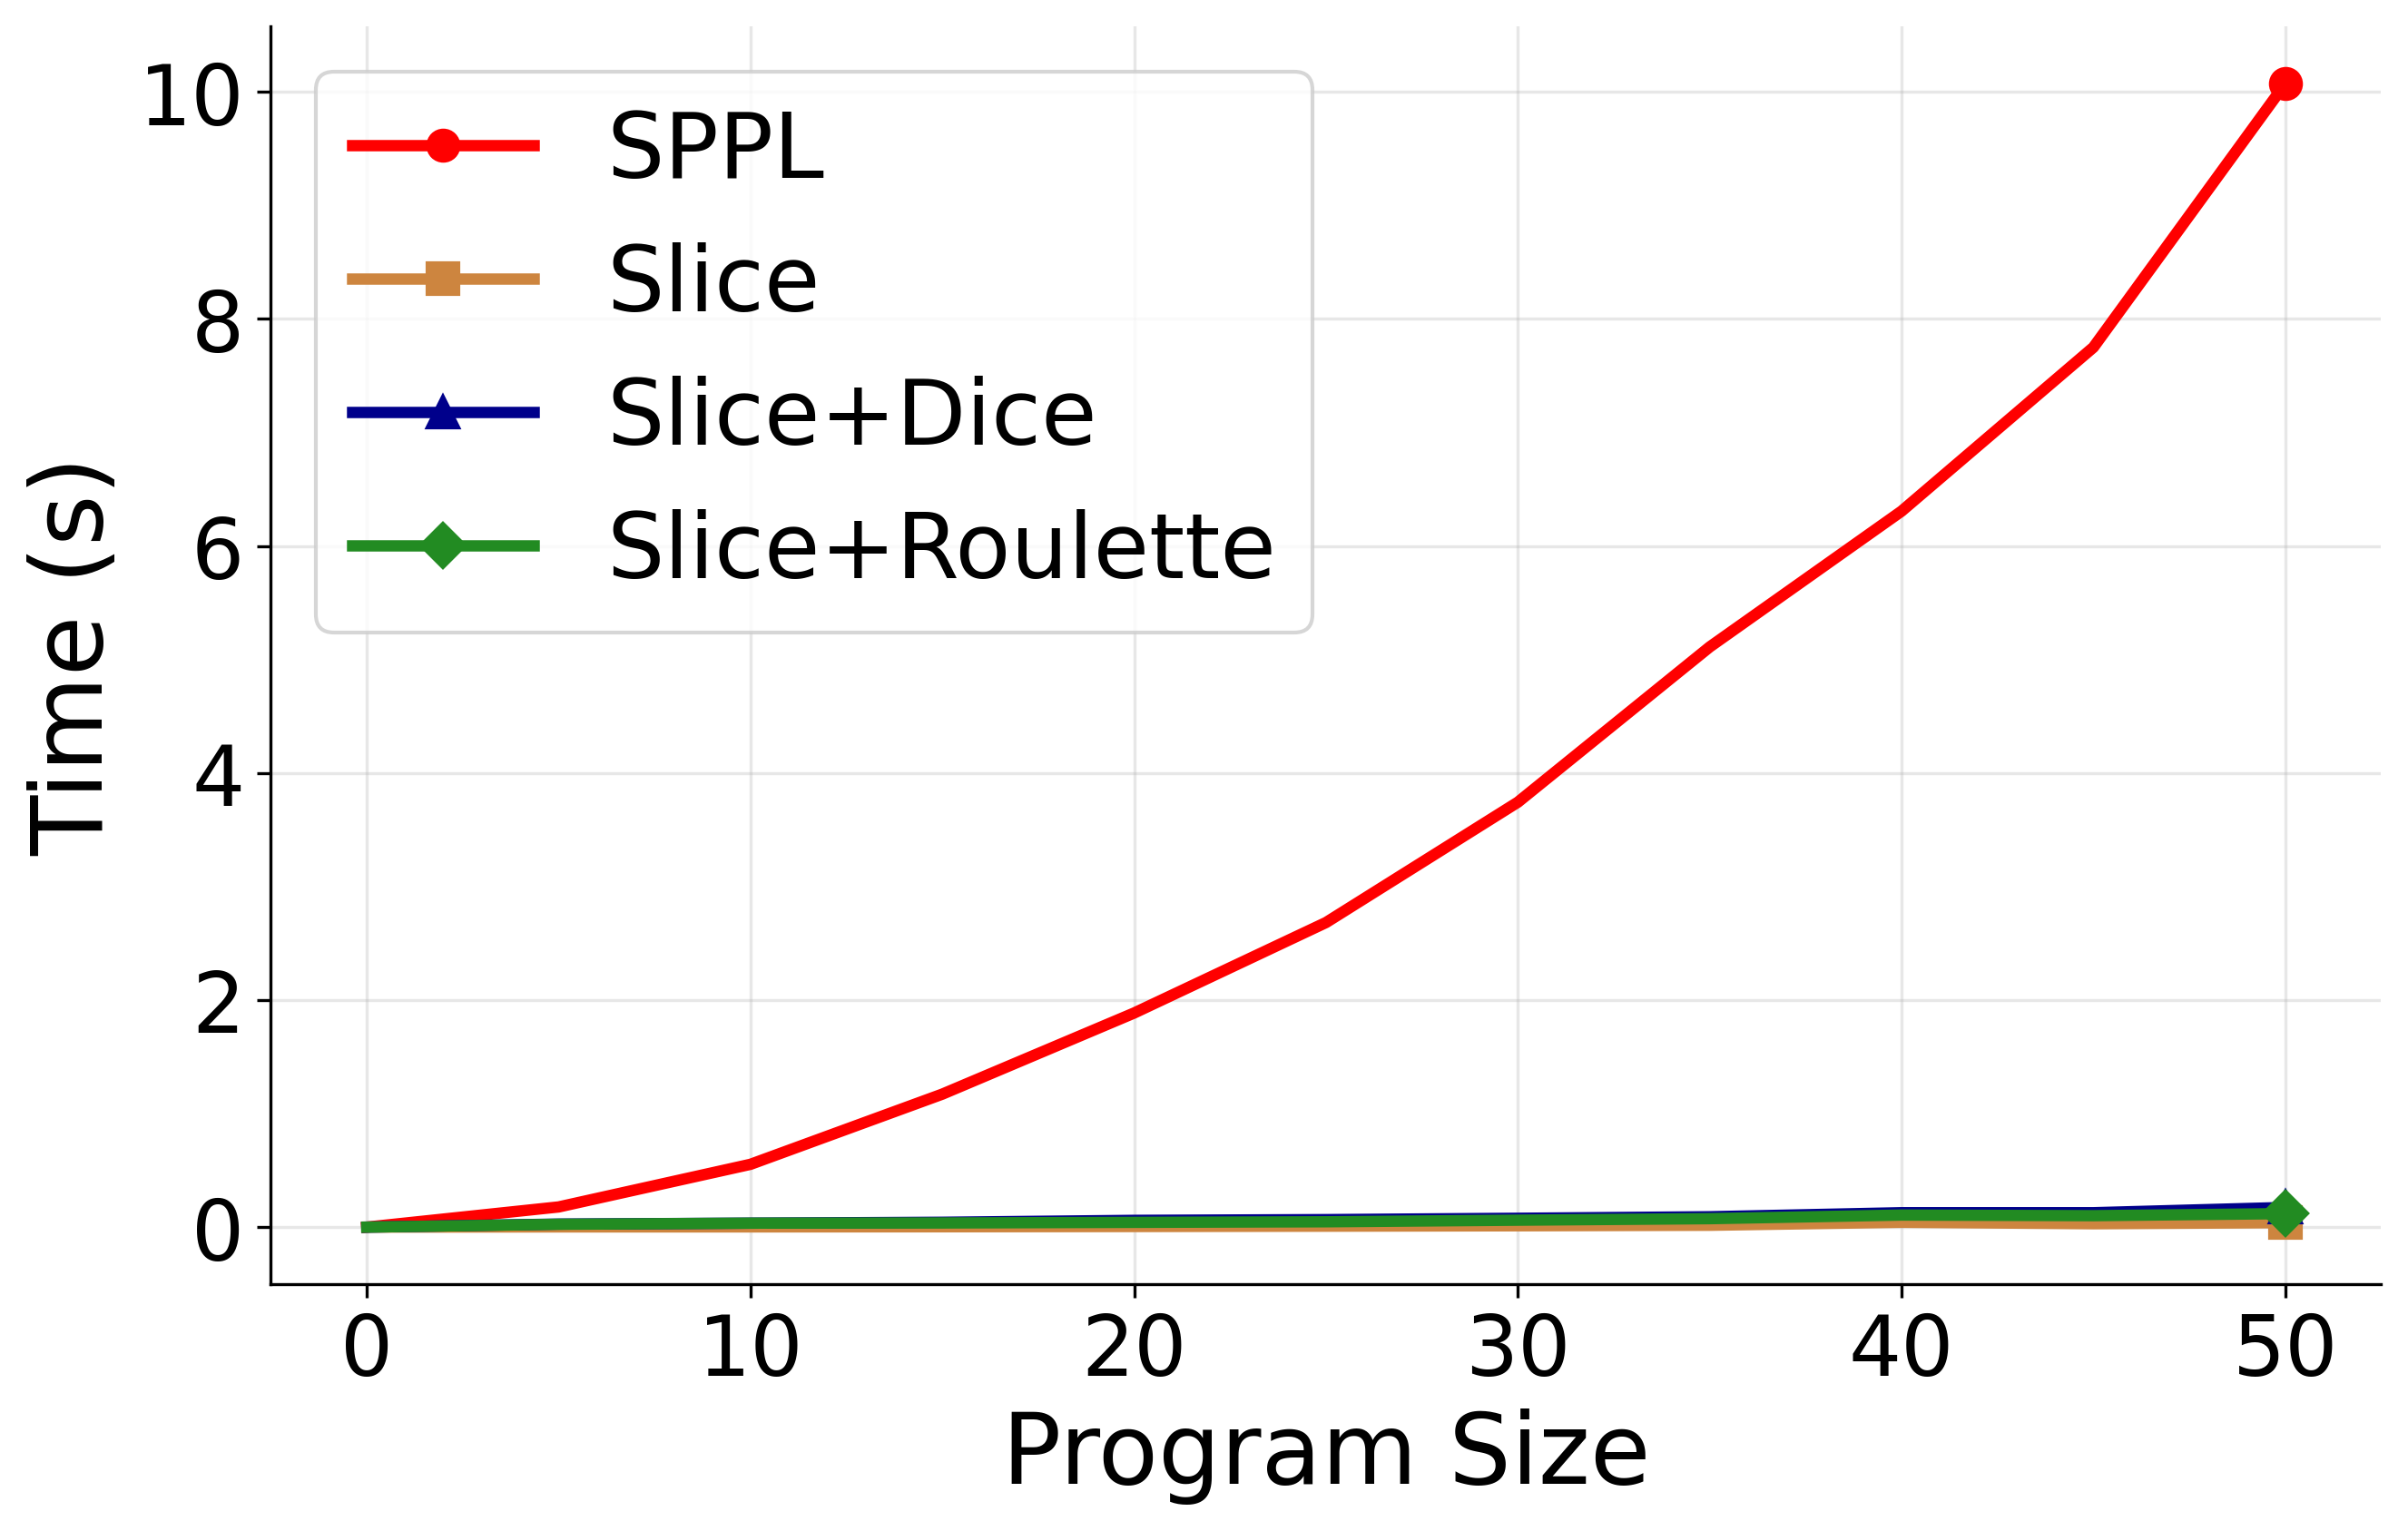
\includegraphics[width=0.98\textwidth]{../images/scaling/build_conditional_independent_fork_slice.png}
        \caption{Cond. Ind. -- Fork}
        \label{fig:cond-benchmarks-b}
    \end{subfigure}
    \hfill
    \begin{subfigure}{0.48\textwidth}
        \centering
        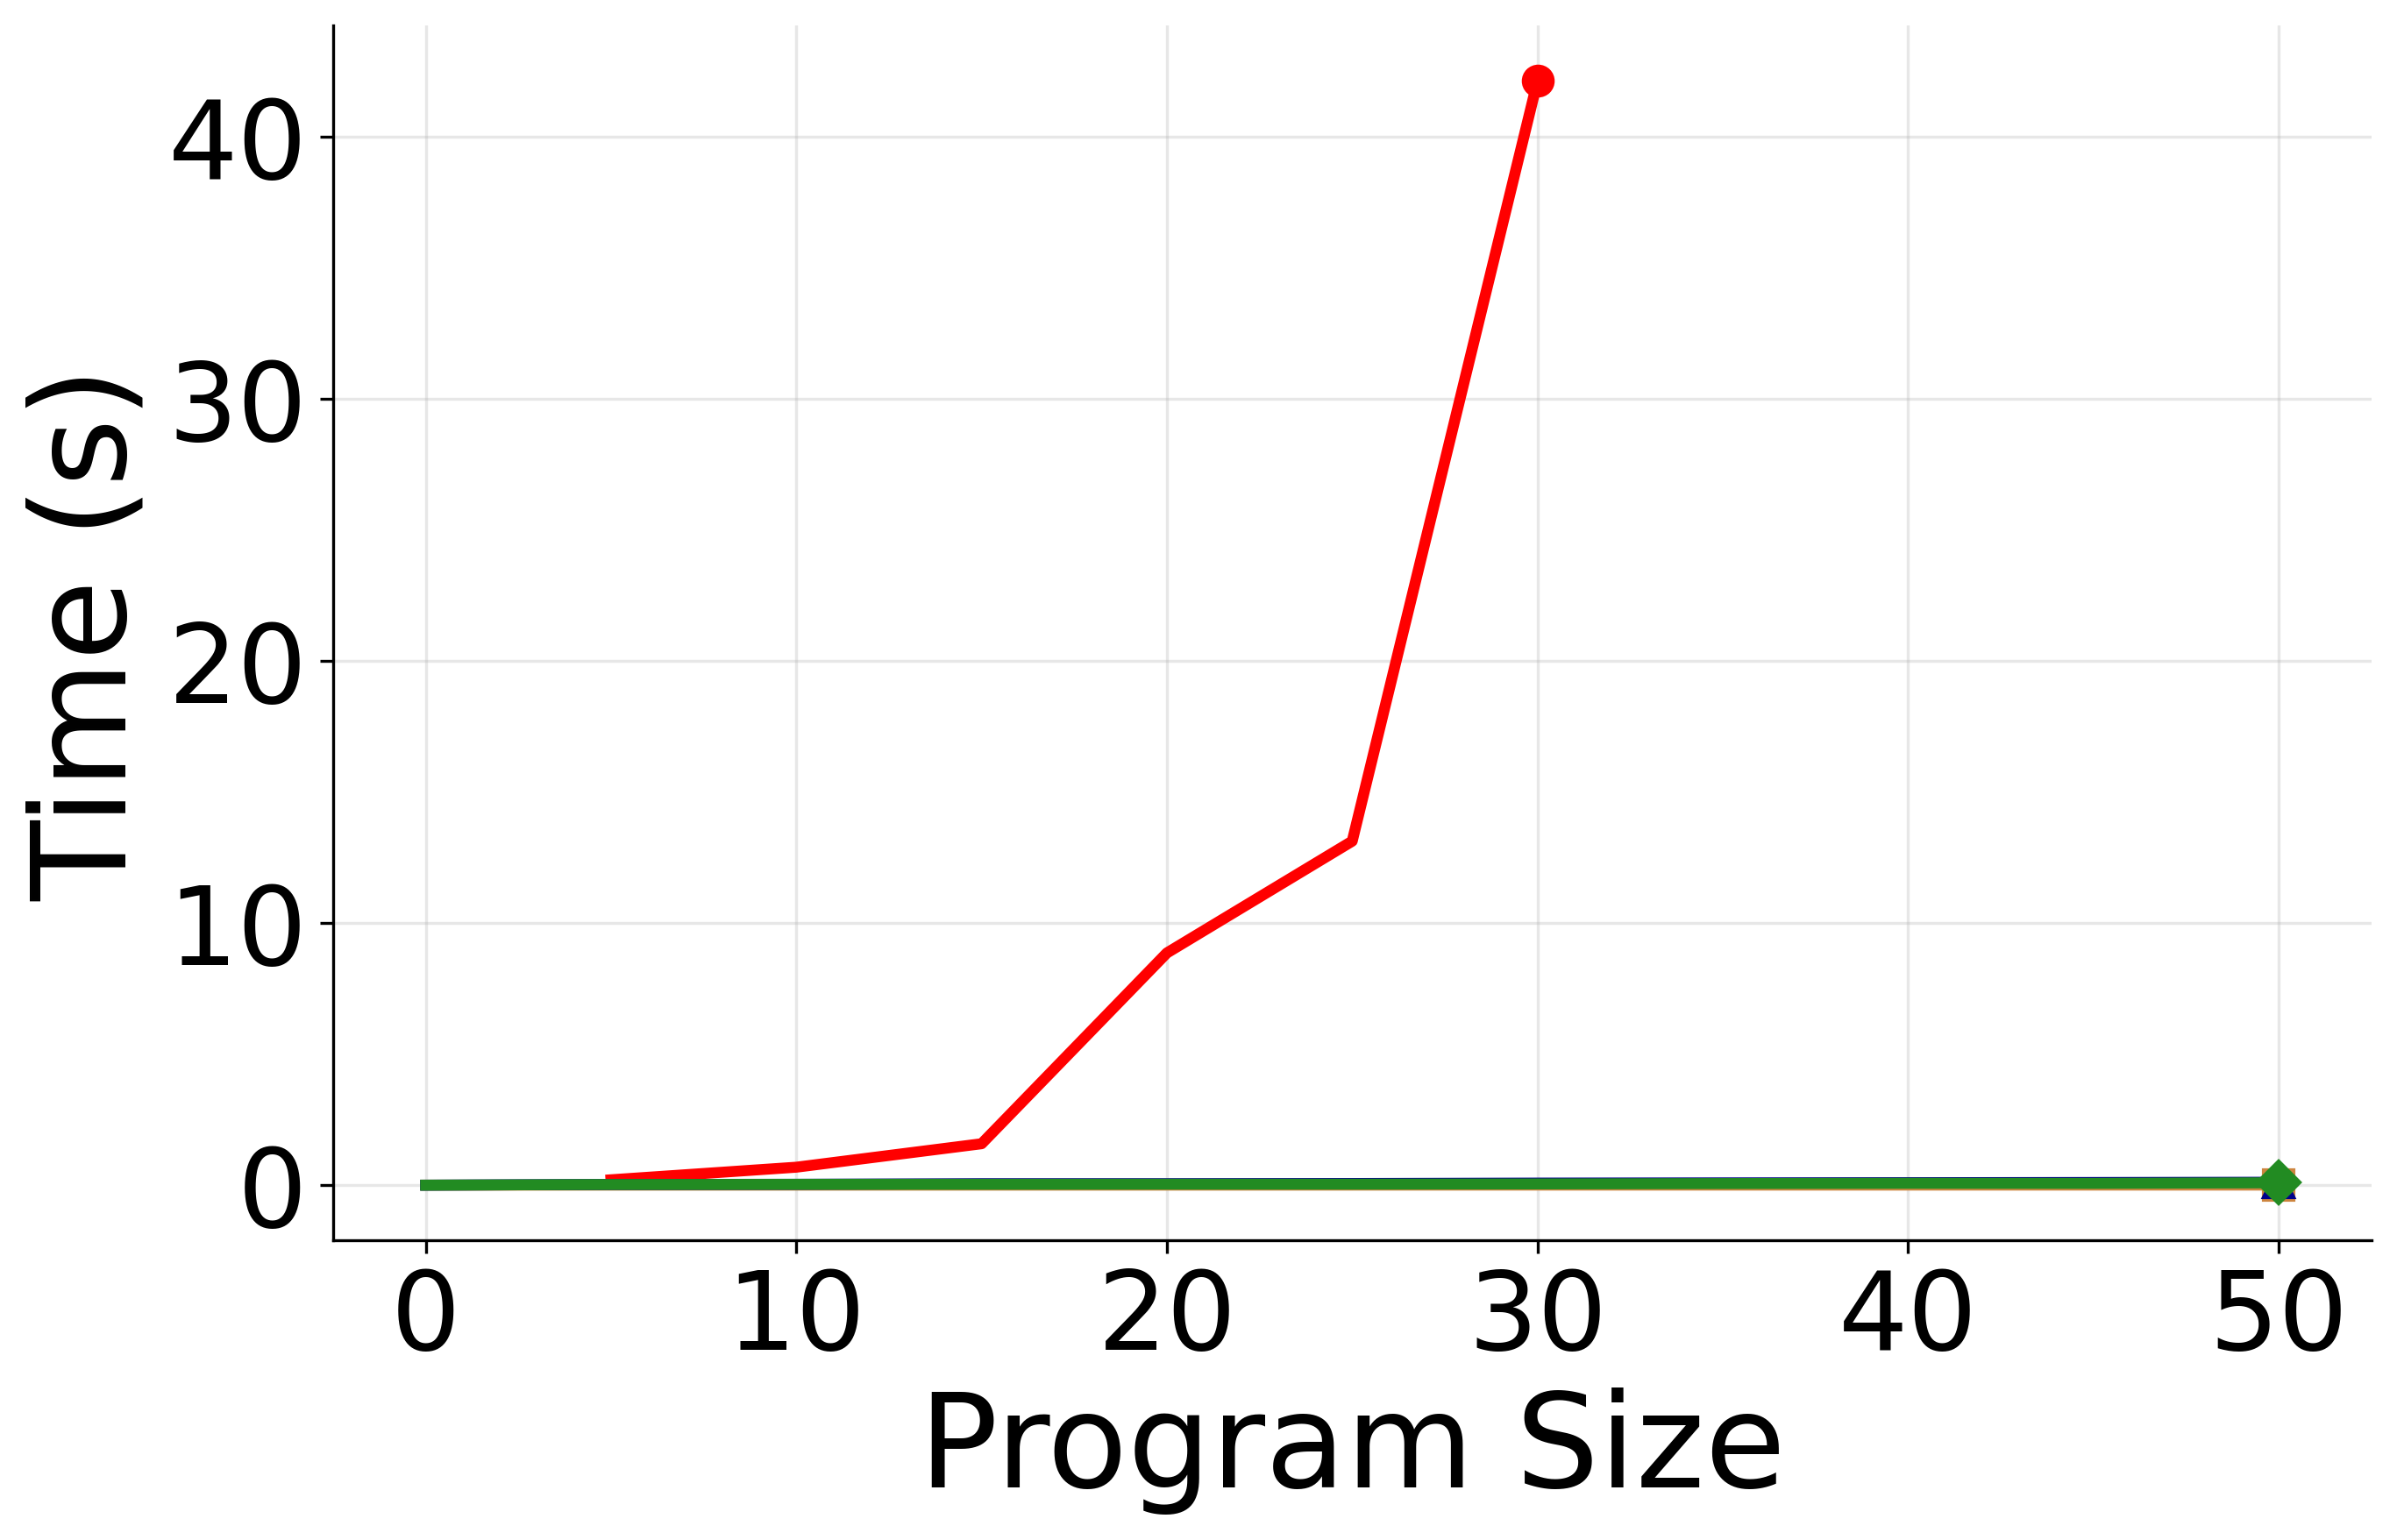
\includegraphics[width=0.98\textwidth]{../images/scaling/build_conditional_random_independent_slice_1.png}
        \caption{Cond. Ind. -- Rand.}
        \label{fig:cond-benchmarks-c}
    \end{subfigure}

    \vspace{1em}

    % Row 2
    \begin{subfigure}{0.48\textwidth}
        \centering
        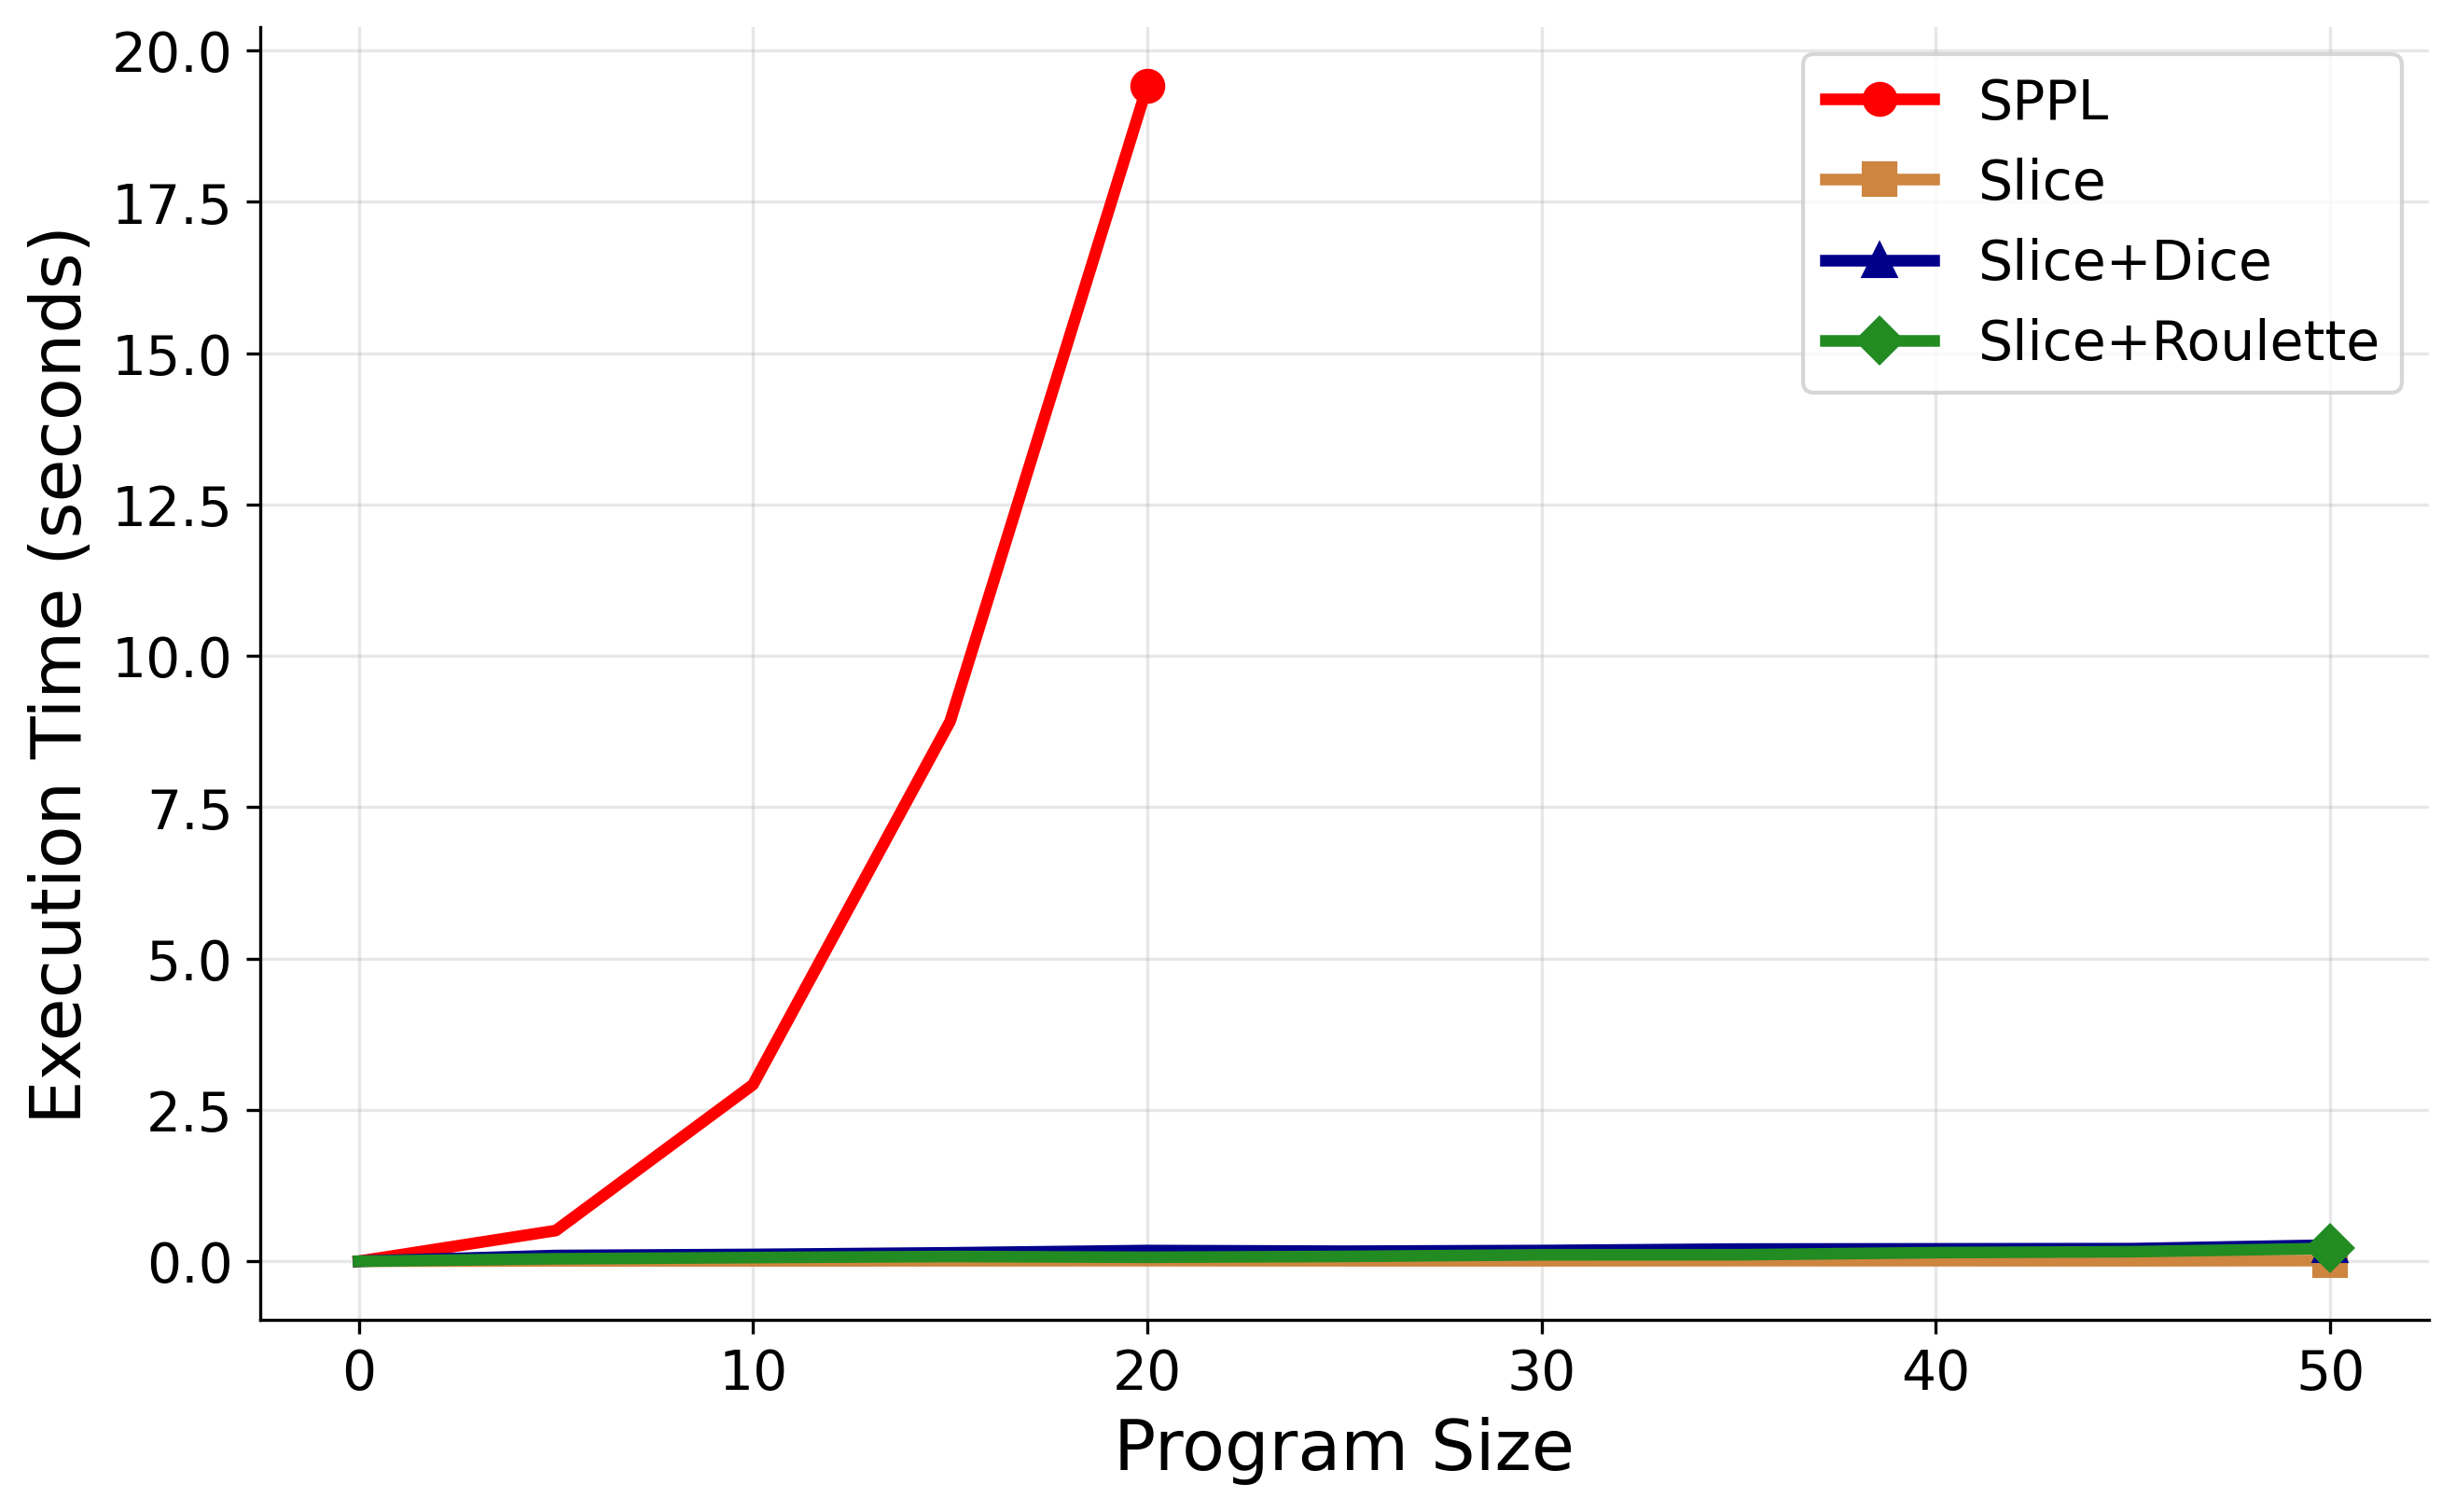
\includegraphics[width=0.98\textwidth]{../images/scaling/build_alternating_guard_slice_1.png}
        \caption{Alt. Guard}
        \label{fig:alt-benchmarks-a}
    \end{subfigure}
    \hfill
    \begin{subfigure}{0.48\textwidth}
        \centering
        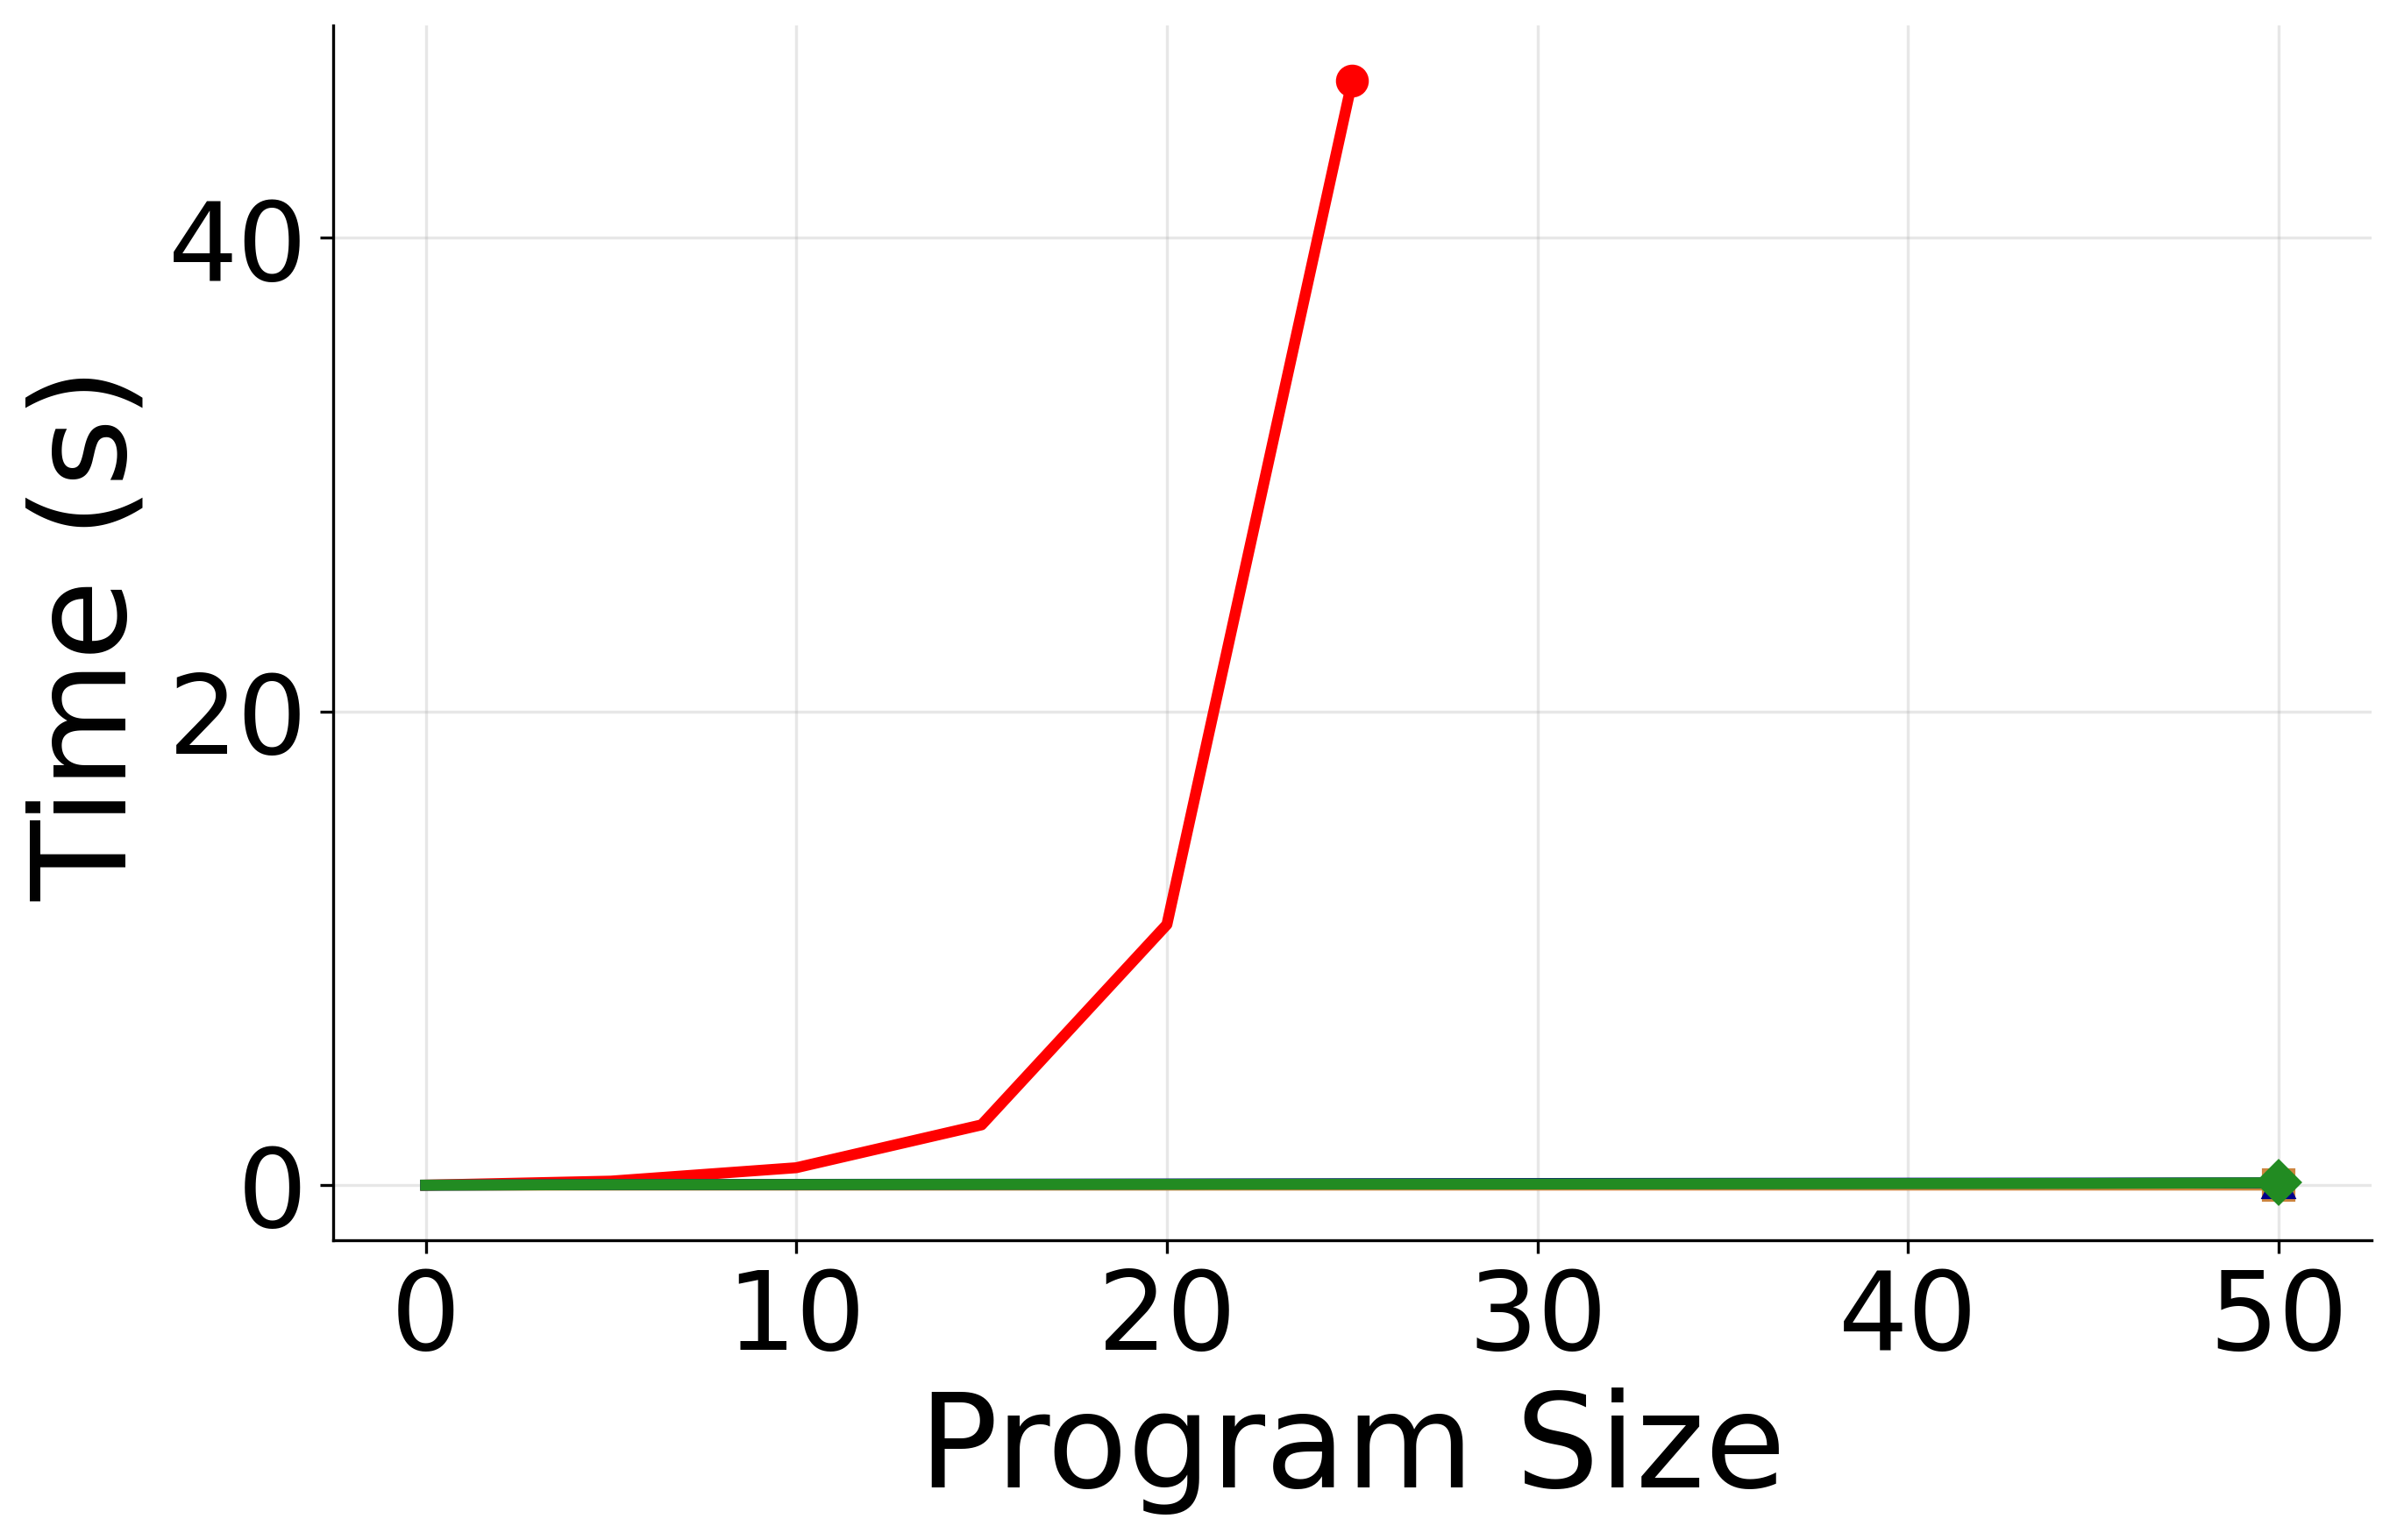
\includegraphics[width=0.98\textwidth]{../images/scaling/build_random_alternating_guard_slice.png}
        \caption{Alt. Guard -- Rand.}
        \label{fig:alt-benchmarks-d}
    \end{subfigure}

    \caption{Results for several scaling benchmarks; the rest are depicted in the Appendix. Time-out=120s. A disappearing line indicates a time-out.}
    \label{fig:alt-benchmarks-main}
    \vspace{-0.2cm}
\end{figure}
